\documentclass[10pt,a4paper]{article}
\usepackage[utf8]{inputenc}
\usepackage[T1]{fontenc}
\usepackage{lmodern}
\usepackage[margin=1.5cm, top=1.4cm, bottom=1.4cm]{geometry}
\usepackage{hyperref}
\usepackage{enumitem}
\usepackage{titlesec}
\usepackage{xcolor}
\usepackage{graphicx}

\definecolor{accent}{HTML}{00686E}
\hypersetup{colorlinks=true, urlcolor=accent, linkcolor=accent}
\pagenumbering{arabic}
\setlength{\parindent}{0pt}

\titleformat{\section}{\large\bfseries\color{accent}}{}{0em}{}[\vspace{-0.6em}\rule{\textwidth}{0.8pt}]
\titlespacing{\section}{0pt}{7pt}{4pt}

\newcommand{\role}[4]{%
  \textbf{#1} \hfill \textbf{#2}\\[1pt]%
  \textit{#3} \hfill \textit{#4}\\[2pt]%
}
\setlist[itemize]{leftmargin=1.2em, itemsep=1.5pt, topsep=2pt, parsep=0pt}

\begin{document}

% ================= HEADER =================
\begin{minipage}[c]{0.80\textwidth}
  {\Huge\bfseries Prabhavit Gupta}\\[3pt]
  {\color{accent}\large AI Engineer: Generative AI, Multi-Agent Systems \& Claude Code}\\[6pt]
  {\footnotesize +39 351 610 7807 ~$\vert$~
  \href{mailto:prabhavitg@gmail.com}{prabhavitg@gmail.com} ~$\vert$~
  \href{https://www.linkedin.com/in/prabhavit/}{linkedin.com/in/prabhavit} ~$\vert$~
  \href{https://github.com/prab-gupta}{github.com/prab-gupta} ~$\vert$~
  Venice, Italy (CET Time Zone / EU Permanent Resident / Unrestricted EU Work Authorization)}
\end{minipage}\hfill
\begin{minipage}[c]{0.18\textwidth}
  \raggedleft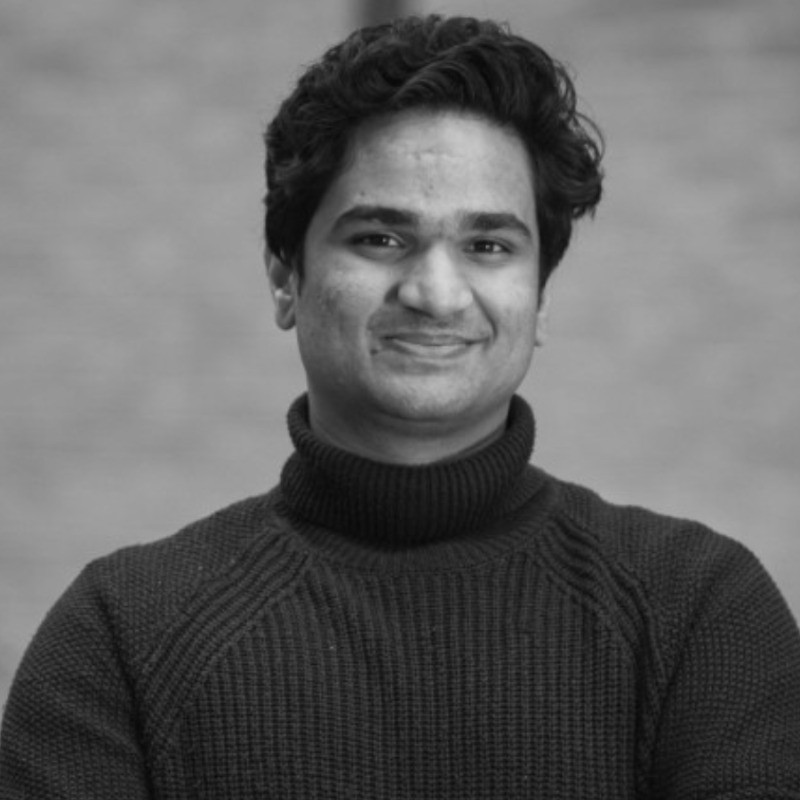
\includegraphics[width=2.0cm]{photo.jpg}
\end{minipage}
\vspace{-2pt}

% ================= SUMMARY =================
\section{Summary}
Applied AI and Data Systems Engineer with 3 years of commercial production experience developing Generative AI applications, autonomous multi-agent loops, and robust Python backend services. Deep hands-on experience integrating frontier LLMs via APIs (Anthropic Claude, OpenAI, Google Gemini) and accelerating software delivery using AI coding agents (Claude Code, Cursor, Antigravity). Skilled in vector databases, embedding generation, semantic search, and building resilient data pipelines that transform enterprise data into production AI capabilities. Based in Venice, Italy (CET time zone) with an EU Long-Term Residence Permit (permanent unrestricted EU work authorization across Spain and all EU member states, no sponsorship required); available immediately for full-time remote roles.

% ================= TECHNICAL EXPERTISE =================
\section{Technical Expertise}
\begin{itemize}
  \item \textbf{Generative AI \& Multi-Agent Systems:} Claude 3.5 Sonnet, GPT-4o, Google Gemini, multi-agent architectures (LangGraph, CrewAI), Model Context Protocol (MCP), tool-calling, reflection loops.
  \item \textbf{AI-Assisted Development Tooling:} Claude Code CLI workflows, Cursor AI, Antigravity agentic harness, prompt engineering, automated prompt evaluation suites.
  \item \textbf{Vector Search \& Embeddings:} Vector databases (Chroma, Qdrant, PGVector), dense embeddings, semantic search, hybrid retrieval, semantic chunking, and Redis caching.
  \item \textbf{Data Engineering \& Backend:} Python (FastAPI, asyncio, Pydantic, requests), PostgreSQL (query optimization, schema modeling), Docker containerization, RESTful APIs, ETL pipelines.
  \item \textbf{Observability \& Quality:} Automated regression testing with pytest and Playwright, structured logging, CI/CD with GitHub Actions.
  \item \textbf{Languages \& Authorization:} English (C1 Professional, fluent), Hindi (Native), Italian (Conversational). EU Long-Term Residence Permit (unrestricted EU work authorization across Spain and all EU member states, no sponsorship required).
\end{itemize}

% ================= EXPERIENCE =================
\section{Experience}

\role{\href{https://flowspace.co}{FlowSpace.co}}{Mar 2024 - Aug 2026}{Lead AI Engineer \& Multi-Agent Architect}{London, UK (remote)}
\begin{itemize}
  \item Architected and deployed enterprise Generative AI applications and multi-agent workflows in Python (FastAPI) serving 4,500+ users with 99.8\% availability.
  \item Integrated LLM APIs (Claude, OpenAI, Gemini) and created custom Model Context Protocol (MCP) servers allowing agents to safely inspect data and execute structured operations.
  \item Accelerated software delivery across the engineering team by integrating Claude Code and Cursor into development lifecycles, cutting feature prototyping time by 50\%.
  \item Implemented semantic search engines and vector retrieval architectures using PGVector and Redis, achieving sub-200ms query latency across complex documentation.
  \item Established automated evaluation pipelines on GitHub Actions to benchmark hallucination rates, token efficiency, and response latency.
\end{itemize}

\role{Urlink}{Apr 2025 - Jul 2025}{Data Platform \& AI Developer (Freelance)}{Barcelona, Spain (remote)}
\begin{itemize}
  \item Developed automated data extraction and transformation pipelines in Python, structuring unstructured datasets into relational databases.
  \item Implemented automated text processing and entity extraction workflows leveraging LLMs and strict Pydantic data models.
  \item Built end-to-end integration test suites with pytest and Playwright to guarantee data accuracy and API contract stability.
\end{itemize}

\role{Independent Technical Consultant}{Aug 2023 - Feb 2024}{Applied AI \& Python Developer}{Venice, Italy}
\begin{itemize}
  \item Developed custom GenAI chatbots, RAG pipelines, and automated reporting microservices for European SMB clients.
  \item Provisioned self-hosted vector stores and backend APIs on cloud Linux instances using Docker.
  \item Authored technical architecture runbooks and developer guidelines for client engineering teams.
\end{itemize}

% ================= EDUCATION =================
\section{Education}
\role{Ca' Foscari University of Venice}{2020 - 2024}{BA in Philosophy, International Studies and Economics}{Venice, Italy}
\begin{itemize}
  \item Rigorous training in formal logic, statistical inference, quantitative economics, and complex systems modeling.
\end{itemize}

\end{document}
